\section{Software used in this project}

Modern astrodynamics and orbital mechanics require the use of numerical routines
and software. In this project, the following software were used:
\href{https://github.com/poliastro/poliastro}{poliastro} and
\href{https://www.ansys.com/products/missions/ansys-stk}{Ansys Systems Tool Kit
(STK)}. All code is hosted in the
\href{https://github.com/jorgepiloto/tfm}{https://github.com/jorgepiloto/tfm}
repository.

The Python library named poliastro focuses on astrodynamics and orbital
mechanics. It provides tools focused on the analysis and design of orbits.
Despite poliastro being archived, the author is a former maintainer of the
project. This allowed the author to build a set of custom numerical routines and
improvements on top of the original source code. Main capabilities from
poliastro include orbit visualization, ephemerides manipulation, and porkchop
plots among many others. For these last figures, their original source code was
parallelized to maximize the performance, reducing computation times.

\vspace{1cm}
\begin{figure}[H] \centering
  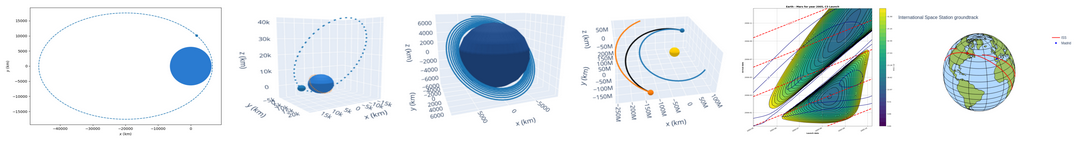
\includegraphics[width=\textwidth]{static/poliastro_capabilities.png}
  \caption[A collection of use cases of poliastro.]{A collection of use
    cases of poliastro. Examples include orbit plotting in 2D and 3D,
    perturbations, and porkchop plots.}
  \label{fig:poliastro_capabilities}
\end{figure}

STK, on the other hand, is a commercial software that provides a set of tools
that extend beyong astrodynamic calculations. It is used for mission analysis,
allowing customers to design, analyze, and visualize complex systems. Its
outstanding performance, accuracy, visualization, and animation capabilities
make this tool a standard in the aerospace industry. Main capabilities used from
STK include validation of results and animations. Regarding animations, these
are presented in the slides acompanying the defense of this project.

\vspace{1cm}
\begin{figure}[H] \centering
  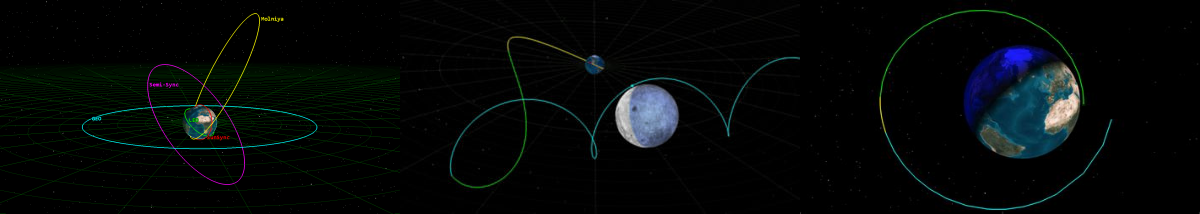
\includegraphics[width=\textwidth]{static/stk_capabilities.png}
  \caption[A collection of use cases of STK.]{A collection of use
    cases of STK. Examples include orbit plotting in 3D, cislunar
    trajectories, and orbit transfer optimization.}
  \label{fig:stk_capabilities}
\end{figure}
